\documentclass[serif,mathserif, 12pt]{beamer}
\usepackage{etex}
\usepackage{amsmath, amsfonts, epsfig, xspace}
\usepackage{algorithm,algorithmic}
\usepackage{pstricks,pst-node}
\usepackage{multimedia}
\usepackage[normal,tight,center]{subfigure}
\setlength{\subfigcapskip}{-.5em}
\usepackage{tkz-euclide}
\usetkzobj{all}
\usepackage{beamerthemesplit}
\usetheme{lankton-keynote}
\usepackage{graphicx,color}
% remove caption of figure
\usepackage[labelformat=empty]{caption}

\usepackage[none]{hyphenat} % hyphenation is ugly in slides
\usepackage{parskip}

\usepackage{relsize} % \smaller to change size

\usepackage{tikz}
\usetikzlibrary{calc}

\usetikzlibrary{arrows}

\newcommand{\TikzDraw}[2][]{
  \begin{tikzpicture}[overlay, remember picture, shift={(current page.center)}, #1]
    #2
  \end{tikzpicture}
}

\newcommand{\gridlines}{
  \TikzDraw{
    \draw[help lines,xstep=.2,ystep=.2,red!20] (current page.south west) grid (current page.north east);
    \draw[help lines,xstep=1,ystep=1,red] (current page.south west) grid (current page.north east);
    \foreach \x in {-15,-14,...,15} {
      \node [anchor=north, red] at (\x,0) {\tiny \x};
      \node [anchor=east,red] at (0,\x) {\tiny \x};
    }
  }
}

\newcommand{\DrawOnImg}[3][]
{
  \begin{tikzpicture}
    \node[anchor=south west,inner sep=0] (image) at (0,0){
      #2
    };
    \begin{scope}[x={(image.south east)},y={(image.north west)}]
      \ifthenelse{\equal{#1}{grid}}
                 {\draw[color=blue, style=dashed] (0,0) grid[xstep=.1, ystep=.1] (1.0001,1.0001);}
                 {}
                 #3
    \end{scope}
  \end{tikzpicture}
}

\usetikzlibrary{matrix}

\newcommand{\BOLD}[1]{\mathbf{#1}}
\newcommand{\BOLDG}[1]{\boldsymbol{#1}}
\newcommand{\PDIF}[2]{\frac{\partial #1}{\partial #2}}
\newcommand{\TODO}[1]{\textcolor{red}{#1}}
\newcommand{\TODOB}[1]{\textcolor{blue}{#1}}
\newcommand{\TODOG}[1]{\textcolor{green!50!black}{#1}}
\newcommand{\argmin}{\operatornamewithlimits{arg\min}}
\DeclareMathOperator{\tr}{tr}
\DeclareMathOperator{\cond}{cond}
\DeclareMathOperator{\ST}{s.t.}
\DeclareMathOperator{\diag}{diag}
\DeclareMathOperator{\Div}{div}

\title[\hspace{2em}\insertframenumber/\inserttotalframenumber]{Mechanical Characterization of Structured Sheet Materials}
\date{28th, September 2018}

\author{Disney Research}

\makeatletter
\let\@@magyar@captionfix\relax
\makeatother

\begin{document}

\maketitle

\begin{frame}
  \frametitle{Isohedral Tillings}
  \TikzDraw{
    \node at (-0.39\textwidth, 0) {
      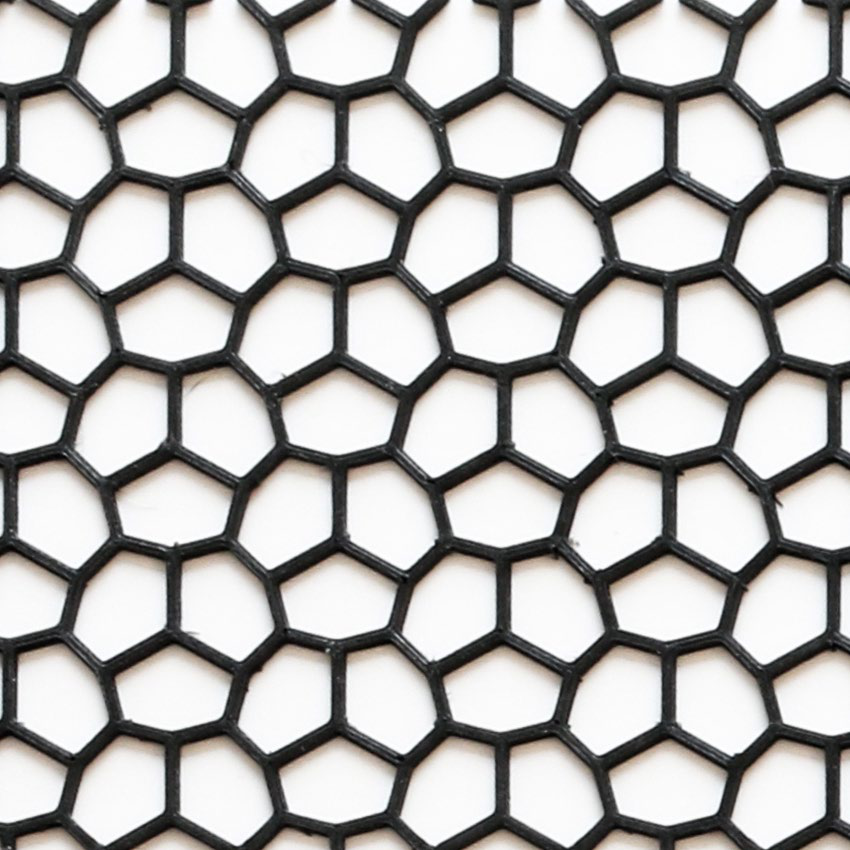
\includegraphics[width=0.25\textwidth]{img/paper-000}
    };
    \node at (-0.13\textwidth, 0) {
      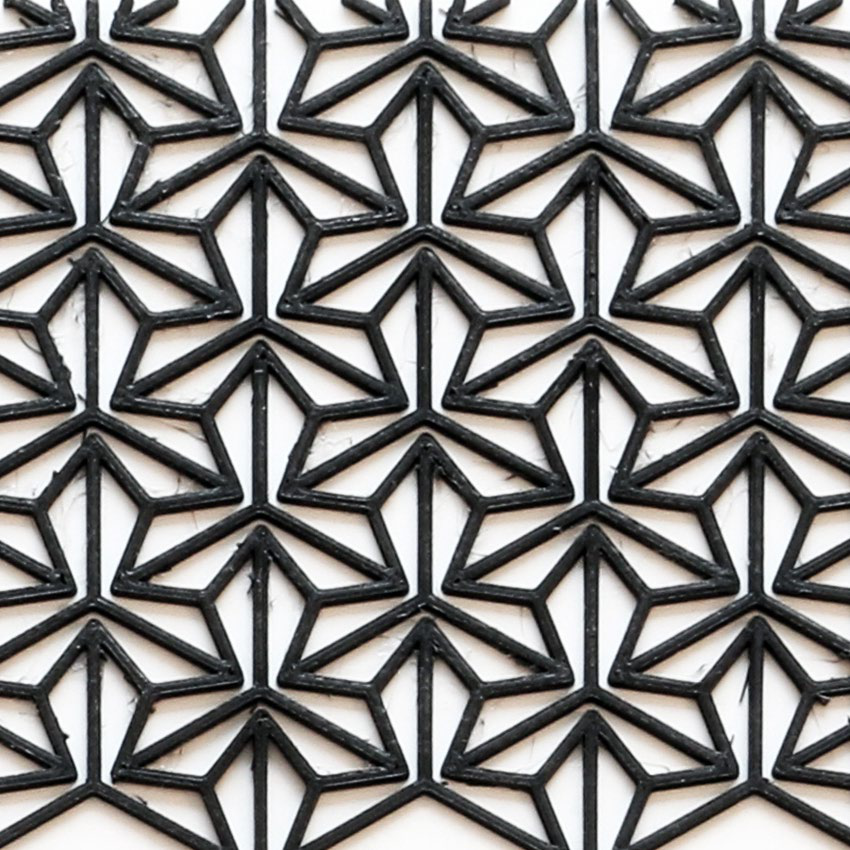
\includegraphics[width=0.25\textwidth]{img/paper-001}
    };
    \node at (0.13\textwidth, 0) {
      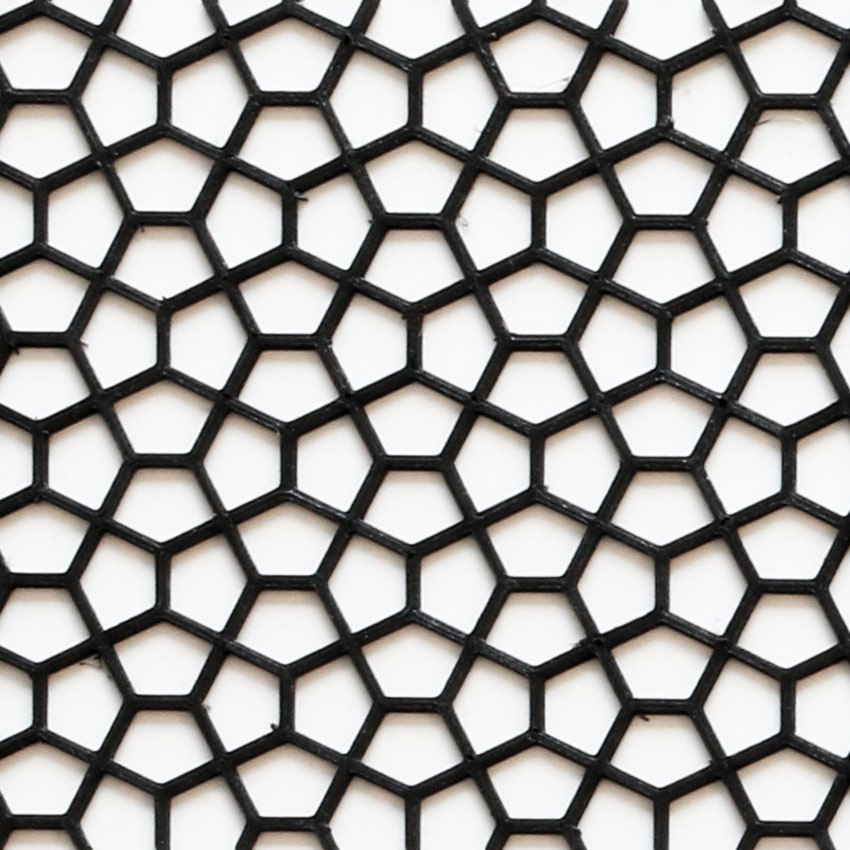
\includegraphics[width=0.25\textwidth]{img/paper-002}
    };
    \node at (0.39\textwidth, 0) {
      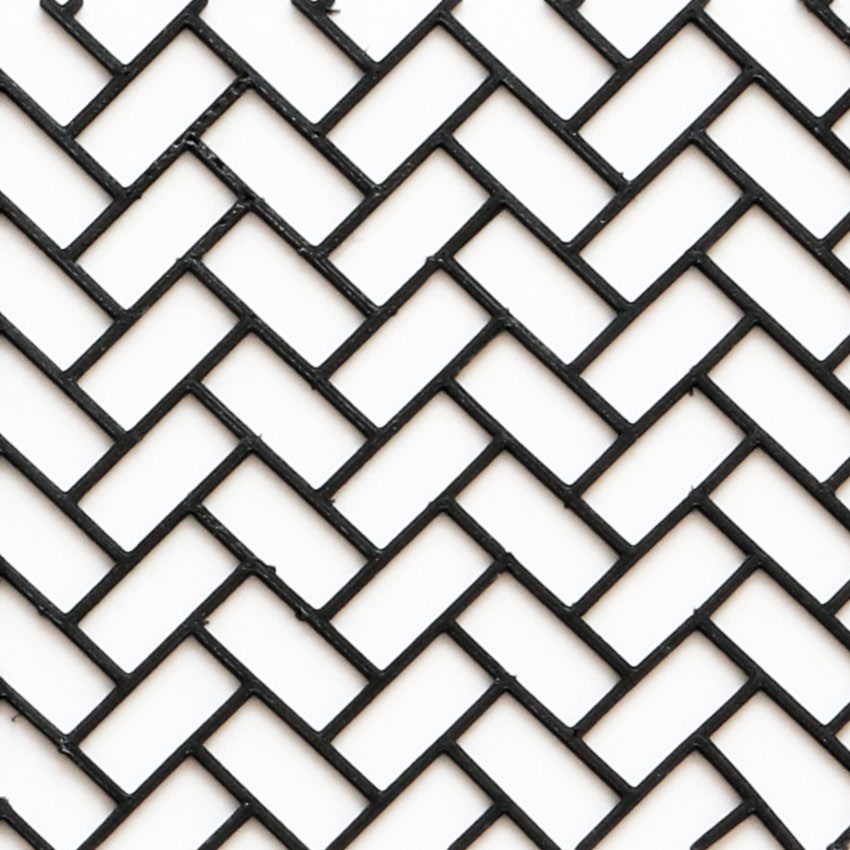
\includegraphics[width=0.25\textwidth]{img/paper-003}
    };
  }  
\end{frame}

\begin{frame}
  \frametitle{Overview}
  
\end{frame}

\begin{frame}
  \frametitle{Mesoscopic Model}
  
\end{frame}

\begin{frame}
  \frametitle{Macroscopic Model}
  \begin{itemize}
  \item Anisotropic Kirchhoff plate
    \begin{equation}
      W(\epsilon, \kappa)
    \end{equation}
  \end{itemize}  
\end{frame}

\begin{frame}
  \frametitle{Homogenization}
  
\end{frame}

\begin{frame}
  \frametitle{}
  
\end{frame}

\begin{frame} 
  \TikzDraw {
    \node at (0, 0.5) {\Huge{Experiments}};
  }
\end{frame}

\begin{frame}
  \frametitle{Inverse structure optimization}
  
\end{frame}

\begin{frame} 
  \TikzDraw {
    \node at (0, 0.5) {\Huge{Thanks!}};
  }
  %\gridlines
\end{frame}

\end{document}
